\hypertarget{Technologie}{\chapter{Technologie}}

\section{Požadavky}

Důležitým uvážením při tvorbě projektu byl výběr licence. Nakonec jsem se rozhodl pro použití licence GNU GPLv3, která je standardem takzvaných copyleft\footnote{Copyleft licence je typem licence pro software a jiný obsah, který umožňuje uživatelům volně používat, upravovat a sdílet software, přičemž vyžaduje, aby všechny odvozené verze byly také licencovány pod stejnými podmínkami. Tím zajišťuje, že software zůstane svobodným.} licencí.

Volba licence je důležitá, protože přímo ovlivňuje, jak se se softwarem může zacházet. GPLv3 mimo jiné zaručuje, že tento projekt navždy zůstane open-source; kdokoliv může prozkoumat, upravit a dále (pod stejnou licencí) sdílet zdrojový kód.\cite{choosealicense}

Dalšími podmínkami byla jednoduchost používání a aktuálnost různých nástrojů, programů a knihoven -- cílem bylo použít moderní (avšak osvědčené), aby program stárnul co možná nejpomaleji.

\subsection{Stack}

Dnes existuje nepřeberně způsobů, jak vytvořit full-stack\footnote{Full-stack označuje kompletní řešení, často za použití serverové i klientské aplikace.} aplikaci a vybrat mezi nimi není jednoduché. Mimoto je tyto technologie potřeba často kombinovat; této kombinaci se nazývá stack. Stack určuje, jak aplikaci vyvíjíme a jaké prostředky nám jsou dostupné. Stack si lze vytvořit sám dle vlastního uvážení a potřeb, nebo využít nějaký volně dostupný, který už je ozkoušený a důvěryhodný.

Mojí volbou se stal \M{T3 Stack}, který kombinuje několik populárních technologií, které jsou blíže popsány níže. Zároveň je však poměrně tvárný a lze ho jednoduše přizpůsobit potřebám projektu.\cite{t3stack}

Jedno z prvních rozhodnutí, které musí člověk při tvorbě projektu udělat je samotný výběr programovacího jazyka. Posledních pár let se většina vývoje soustředí kolem jazyka \M{TypeScript}, který je typovanou\footnote{Typy v programovacím jazyce definují struktury, ve kterých se mimo jiné dají ukládat data. Pokud předem víme, jak tyto struktury vypadají, dá se jednodušeji při programování vyhnout chybám.} variantou jazyka \M{JavaScript}. \M{T3 Stack} ho automaticky používá. 

Framework je jakási nadstavba nad programovacím jazykem a má proces vytváření webových aplikací usnadnit. Při tvorbě webové aplikace fungují jako páteř, na které stojí vše ostatní. \M{T3 Stack} přichází s frameworkem \M{Next.js}, který je sám o sobě nadstavbou nad populárním frameworkem \M{React}. Nabízí mnoho funkcí, jmenovitě například možnost výběru stylu renderování stránky, automatické optimalizace a různé další funkcionality.\cite{nextjs}

Databáze je další klíčovou součástí jakékoli větší aplikace. Pro tento projekt jsem zvolil \M{PostgreSQL}; jedná se o jeden z nejvšestranějších volně dostupných databázových systémů.

\M{T3 Stack} přichází s knihovnou \M{Prisma}, která komunikaci s databázi usnadňuje například tím, že pro TypeScript generuje typy podle definovaného schéma.

Na rozdíl od jiných populárních CSS frameworků, jako je například \M{Bootstrap} nebo \M{Skeleton} se \M{TailwindCSS} liší tím, že nenabízí již předem připravené komponenty, ale pouze profesionály definované CSS třídy. Vývojář díky tomu není žádným způsobem omezován.\footnote{Navíc, pokud je člověk ve tvorbě webů zběhlý, na první pohled dokáže poznat připravené komponenty z populárních CSS  frameworků, což je vzhled, kterému jsem se chtěl vyvarovat.} \M{TailwindCSS} je automaticky obsažen v \M{T3 Stack}u.

Autentifikace je při tvorbě webových aplikací častým úskalím, proto \M{T3 Stack} automaticky přichází s \M{NextAuth.js}, což je rozšíření pro použitý framework \M{Next.js}. Umožňuje přihlašování s Google účtem, což je pro tuto aplikaci potřeba. Jedná se o léta používaný standard, což je u což je u bezpečnostně kritického komponentu jedna z žádaných vlastností. Zároveň jsou všechny kritické bezpečnostní chyby hlášeny na amerických státních stránkách NIST.

Sestavený kód je spouštěn pomocí \M{Node.js} za pomocí balíčkovacího programu \M{NPM}. Zároveň je možné celý program spolu s databázovým systémem spustit v \M{Docker} kontejnerech.

Program je verzován pomocí verzovacího systému \M{Git}.

Všechny výše zmíněné technologie jsou dostupné pod open-source licencemi.

\section{Program}

Program je poměrně rozsáhlý, proto je pro přehlednost rozdělen do několika souborů a složek. Všechny konfigurační soubory se nacházejí v kořenové cestě aplikace. Všechny soubory týkající se databáze, včetně migrací\footnote{Migrace je sql soubor který definuje postupné změny databáze během vývoje.} a schématu, jsou ve složce \M{/prisma/}. Všechny statické soubory, jako jsou například obrázky a ikony jsou ve složce \M{/public/} (toto je složka, kterou \M{Next.js} automaticky detekuje a všechny soubory uvnitř ní zveřejní v sestavené verzi aplikace). Složka \M{/src/} obsahuje samotný zdrojový kód.

\subsection{Konfigurace}
\label{sec:config}

Protože je v programu použito hodně nástrojů, je potřeba mnoha konfiguračních souborů.

\M{package.json} definuje použité knihovny a různé scripty\footnote{Script je typicky malý kus kódu, který nijak nezasahuje do funkčnosti aplikace, ale vypomáhá při jejím vývoji.}; tento soubor využívá balíčkovací systém \M{NPM} při instalaci potřebných balíčků. \M{tailwind.config.cjs}, \M{prettier.config.cjs} a \M{postcss.config.cjs} nastavují funkčnost \M{Tailwind}u. \M{next.config.mjs} a \M{next-env.d.ts} konfigurují funkčnost \M{Next.js}. Soubor \M{.gitignore} definuje, jaké soubory má \M{Git} ignorovat.

Konfigurace samotného programu je uložena v souboru \M{.env}. Tento soubor není v repozitáři přítomen, protože obsahuje citlivé informace (přístupové údaje k databázi aj.); místo toho je přítomen soubor \M{.env-example}, kde jsou všechny nastavitelné hodnoty popsány a nevyplněny. Níže následuje úryvek z tohoto souboru.

\indent

\hrule
\begin{verbatim}
# VARIABLE INFO
NEXT_PUBLIC_SUBTITLE="Rozřazovací testy pro [jméno školy]"
NEXT_PUBLIC_REPOSITORY="https://github.com/chamik/rozrazovak"
NEXT_PUBLIC_CONTACT_EMAIL="aktualni-administrator@example.org"

# Teacher email adresses (comma separated)
TEACHER_EMAILS=ucitel@gjp-me.cz,obcan-k@email.cz

# Prisma
POSTGRES_USER=postgres
POSTGRES_PASS=supertajneheslo
POSTGRES_DB=rozrazovak

# Next Auth Google Provider
GOOGLE_CLIENT_ID=
GOOGLE_CLIENT_SECRET=
\end{verbatim}
\hrule

\subsubsection{Docker}

Pro usnadnění spouštění programu lze projekt spustit v Docker kontejneru. Soubor \M{Dockerfile} definuje, jak program sestavit a spustit. Soubor \M{docker-compose.yml} poté definuje, jak se má spustit databáze spolu s programem a jak mezi sebou komunikují. \cite{docker}

Script \M{start.sh} provádí podle nastavení při každém spuštění migrace a končeně spouští program.

\subsection{Databáze}

Schéma databáze je definované pomocí souboru \M{prisma/schema.prisma}. Obsahuje definice uživatelů, testů, odpovědí, aktuálních přihlášení aj. (vizte obrázek \ref{schema}) Jedná se o soubor se speciálním zápisem, který následně \M{Prisma} používá k vytváření SQL migrací, Typescript typů atd. Díky této funkcionalitě v programu není ani jeden ručně psaný řádek SQL kódu.

Výhodou tohoto přístupu je, že \M{Prisma} dokáže převádět tento obecný zápis a dotazy na specifické verze SQL podle použité databáze. \cite{prisma} Níže následuje úryvek schématu.

\indent

\hrule
\begin{verbatim}
model Question {
    id            Int          @id @default(autoincrement())
    languageLevel Int          @default(0)
    questionText  String       @default("")
    rightAnswer   String       @default("")
    wrongAnswers  String[]     @default(["", "", ""])
    questionType  QuestionType @default(GRAMMAR)
    pointAmount   Int          @default(1)

    answers Answer[]
}

enum QuestionType {
    GRAMMAR
    READING
    LISTENING
}
\end{verbatim}
\hrule

\begin{figure}[H]
    \centering
    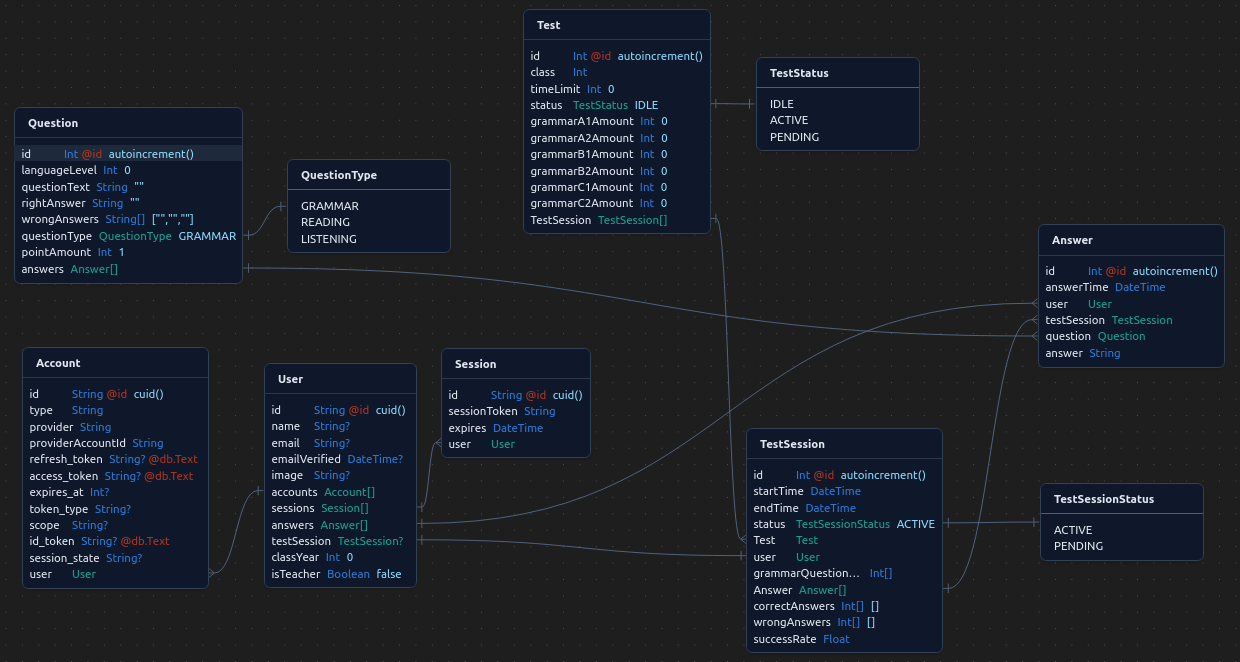
\includegraphics[width=420px]{images/02technologie/schema.png}
    \caption{Vizualizované schéma databáze. Každý modrý blok popisuje jednu tabulku. V tabulce se nachází jména sloupců společně s jejich typy. Šedé čáry značí relace.}
    \label{schema}
\end{figure}

Během vývoje se schéma databáze měnilo. Při každé změně byla vytvořena migrace, která změnu přesně popisuje. Díky tomu lze program vracet do různých fází vývoje a aktualizovat živou\footnote{Takzvaná živá databáze je databáze s produkčními daty. Při vývoji se používá databáze lokální, aby případně nedošlo ke katastrofické ztrátě dat.} databázi bez větších problémů. Všechny migrace se nachází ve složce \M{prisma/migrations/}.

\subsection{Přihlašování}
\label{sec:login}

Boilerplate\footnote{Boilerplate je opakující se nebo standardní kód, který je často používán v různých částech softwaru a aplikací. Jedná se o kód, který obsahuje základní strukturu a funkce.} kód pro přihlašování přichází s \M{T3 Stack}em už připravený, je však upraven tak, aby vyhovoval požadavkům projektu -- specificky aby aplikace umožňovala přihlašování se školním Google účtem.

Specifická implementace se nachází v \M{src/pages/api/auth/[...nextauth].ts}. Při přihlášení si program kontroluje použitou e-mail adresu -- nejdříve pokud se nachází v seznamu učitelů (vizte \ref{sec:config}), v takovém případě uživateli přidělí roli učitele s přístupem do učitelského rozhraní (vizte \ref{sec:admin}). 

Pokud ne, program se ujistí, že je e-mail součástí školní domény. Poté je díky specifické konvenci GJP-ME dávat žákům e-mailové adresy ve formátu \M{[rok nástupu na školu][typ studia][pořadí žáka v abecedním seznamu]@gjp-me.cz} schopen získat rok nástupu žáka a podle toho vypočítat, v jakém ročníku se aktuálně nachází (vizte níže). Všechny tyto údaje jsou uloženy do databáze.

\indent

\hrule
\begin{verbatim}
function parseUserLevel(email: string) {
    const emailId = email.split('@')[0];
    
    const date = new Date();
    const currentYear = date.getFullYear();
    const currentMonth = date.getMonth();
    
    const userYear = 2000 + parseInt(emailId!.slice(0, 2)!);
    
    let level = 0
    if (emailId?.slice(2, 4) == '08')
        level = currentYear - userYear;
    else
        level = currentYear - userYear + 4;
    
    if (8 <= currentMonth && currentMonth <= 11 )
        level += 1;
    
    return level;
}
\end{verbatim}
\hrule

Pro bylo přihlašování přes Google účet možné, je potřeba svoji aplikaci registrovat v Google Developer Console. Zde je možné editovat, k jakým údajům uživatele má aplikace přístup (v tomto případě pouze ke jménu a e-mailu), název aplikace zobrazený uživateli aj. Také je zde potřeba správně nastavit callback adresu -- kam Google uživatele přesměruje po přihlášení -- a potvrzené zdroje JavaScriptu.

\begin{figure}[H]
    \centering
    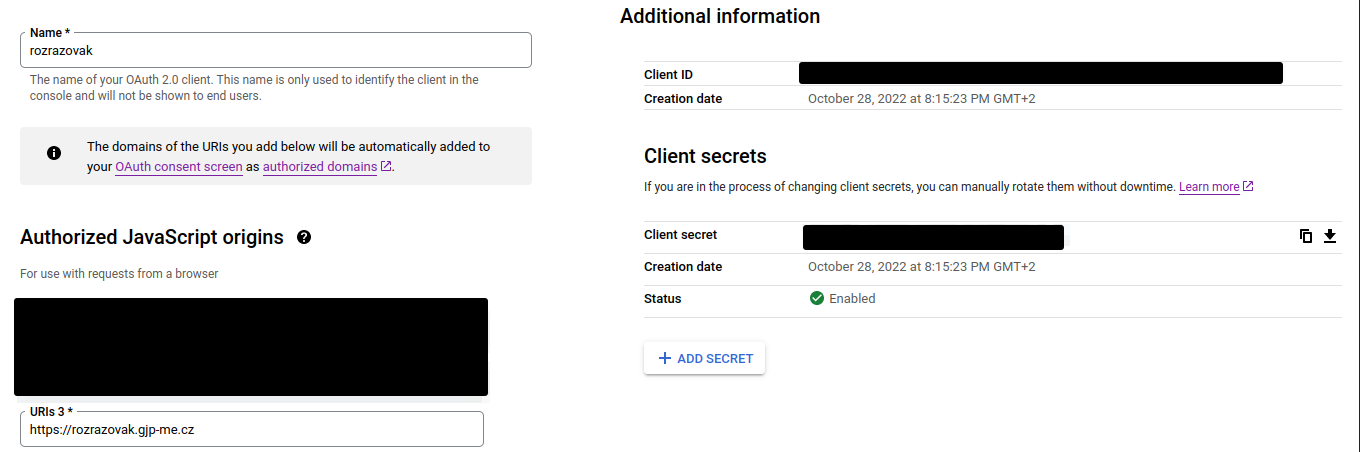
\includegraphics[width=420px]{images/02technologie/google-console.png}
    \caption{Redigovaný snímek obrazovky z Google Developer Conosle.}
\end{figure}

Po správném nastavení a potvrzení administrátorem organizace podle použité domény aplikace je na této stránce možné získat \M{CLIENT\_ID} a \M{CLIENT\_SECRET}, které je potřeba vyplnit v konfiguračním souboru aplikace (vizte \ref{sec:config}).

K potvrzení identity uživatele se používá protokol OAuth 2.0, který \M{NextAuth.js} automaticky zpracuje a vývojáři zpřístupní relevantní údaje, jako je například právě e-mail a jméno.

\begin{figure}[H]
    \centering
    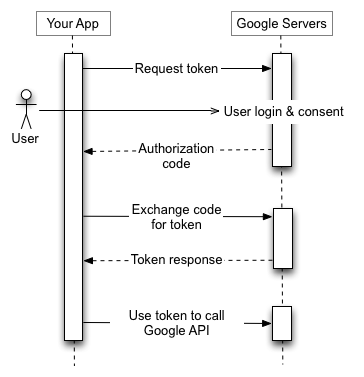
\includegraphics[width=200px]{images/02technologie/google-auth.png}
    \caption{Schéma komunikace aplikace se servery Googlu během přihlašování. Sdíleno Googlem. \cite{google-auth}}
\end{figure}

Pokud celý tento proces proběhl úspěšně, je uživatel přesměrován zpět na hlavní stránku (vizte \ref{sec:login-design}). Pokud ne, uživateli je sděleno, že přihlašování neproběhlo úspěšně.

\section{Nasazení}

Program je potřeba někde spustit tak, aby byl dostupný na internetu. Pro tento účel jsem zvolil služby společnosti Hetzner, které nabízejí VPS\footnote{Virtual Private Server, nebo česky virtuální soukromý server} za rozumné ceny a mám s nimi již dobré zkušenosti. 